%%% PREAMBLE - Do not touch %%%%%%%%%%%%%%%%%%%%%%%%%%%%%%%%%%%%%%%%%%%%%%%%%%%%%%
\documentclass[10pt,twocolumn,letterpaper]{article}
\usepackage[utf8]{inputenc}
\usepackage[english]{babel}
\usepackage{model}
\usepackage{times}
\usepackage{epsfig}
\usepackage{graphicx}
\usepackage{amsmath}
\usepackage{textcomp}
\usepackage{amssymb}
\usepackage{color}
\usepackage[pagebackref=true,breaklinks=true,letterpaper=true,colorlinks,bookmarks=false]{hyperref}

%% inset source code
\usepackage{listings}

\lstset{basicstyle=\footnotesize\ttfamily,  language=C}
\renewcommand{\lstlistingname}{Code}% Listing -> Algorithm

\let\url\nolinkurl% Make \url be equivalent to \nolinkurl
\newcommand*{\Package}[1]{\texttt{#1}}%

\cvprfinalcopy % *** Uncomment this line for the final submission
\def\httilde{\mbox{\tt\raisebox{-.5ex}{\symbol{126}}}}
\ifcvprfinal\pagestyle{empty}\fi

\newcommand{\TODO}[1]{TODO: #1}
\newcommand{\CITEONE}[2]{\mbox{#1 \cite{#2}}}
\newcommand{\CITETWO}[3]{\mbox{#1 and #2 \cite{#3}}}
\newcommand{\CITEN}[2]{\mbox{#1 et al. \cite{#2}}}

%%% Report beginning %%%%%%%%%%%%%%%%%%%%%%%%%%%%%%%%%%%%%%%%%%%%%%%%%%%%%%%%%%%%%%
\begin{document}

%%% Title and authors %%%%%%%%%%%%%%%%%%%%%%%%%%%%%%%%%%%%%%%%%%%%%%%%%%%%%%%%%%%%
\title{Relatório da atividade 2.2}
\author{Isadora Sophia Garcia Rodopoulos \thanks{RA 158018, Instituto de Computação, Universidade de Campinas, Unicamp. \textbf{Contact}: \tt\small{isadorasophiagr@gmail.com}} \\
Matheus Mortatti Diamantinos \thanks{RA 156740, Instituto de Computação, Universidade de Campinas, Unicamp. \textbf{Contact}: \tt\small{matdiamantino@gmail.com}}\\
Luiz Fernando Bittencourt\thanks{MC833, Instituto de Computação, Universidade de Campinas, Unicamp. \textbf{Contact}: \tt\small{bit@ic.unicamp.br }}\\
}

%%% Abstrato %%%%%%%%%%%%%%%%%%%%%%%%%%%%%%%%%%%%%%%%%%%%%%%%%%%%%%%%%%%%%%%%%%%%%
\maketitle
\begin{abstract}
O objetivo do trabalho se baseou em modificar a implementação da aplicação cliente-servidor
anterior, substituindo \texttt{fork()} por \texttt{select()}.
\end{abstract}

%%% image for demo! %%%%%%%%%% 
\begin{figure*}
\begin{center}
    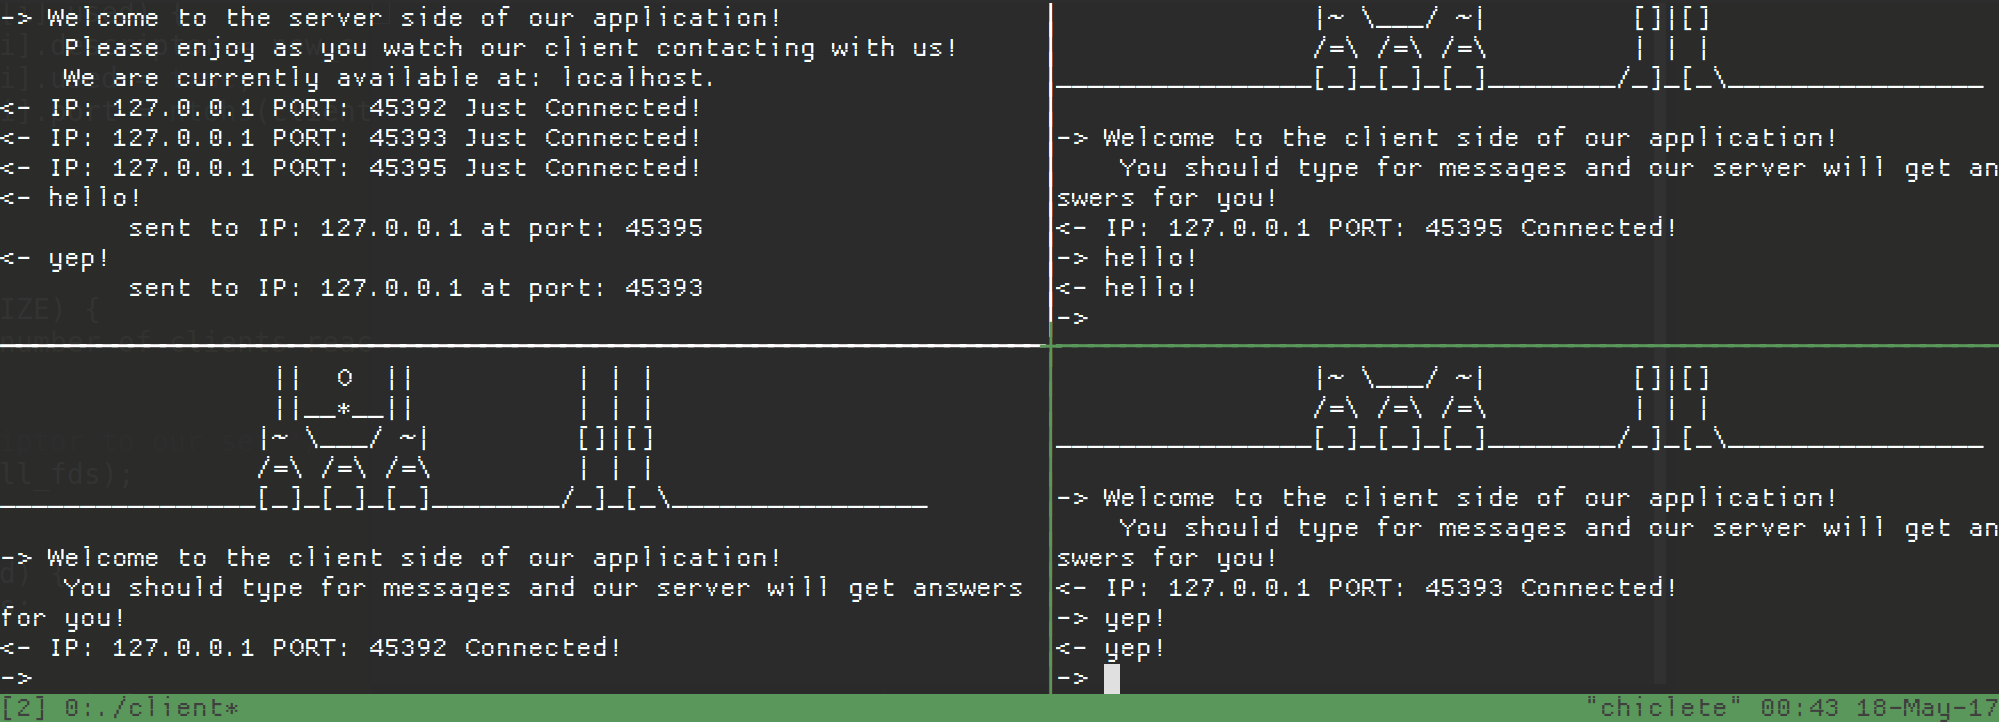
\includegraphics[width=1\textwidth]{img/sample.png}
    \caption{Exemplo de funcionamento do projeto}   
\end{center} 
\end{figure*}
%%%%%%%%%%%%%%%%%%%%%%%%%%%%%%%%%% page 2

%%% Introdução %%%%%%%%%%%%%%%%%%%%%%%%%%%%%%%%%%%%%%%%%%%%%%%%%%%%%%%%%%%%%%%%%%%
Neste projeto, foi implementado uma estrutura de comunicação entre cliente e servidor baseado em uma conexão TCP utilizando sockets na linguagem C. Nela, vários clientes podem se conectar a um mesmo IP, cada um por uma porta diferente. Foi utilizada a estrutura de \texttt{select()} para permitir que vários clientes se conectem simultaneamente.

Além disso, um \textit{ack} é enviado para cada um dos clientes, em formato de \textit{echo}, para certificar que a mensagem chegou com sucesso.

%%% Seções %%%%%%%#####%%%%%%%%%%%%%%%%%%%%%%%%%%%%%%%%%%%%%%%%%%%%%%%%%%%%%%%%%%%
\section{client.c}
O código para o cliente não sofreu nenhuma modificação em relação aos projetos anteriores,
uma vez que o seu comportamento continua o mesmo, basta conectar-se ao IP do servidor e 
a uma porta disponível.

O fluxo de execução de \texttt{client.c} pode ser resumido, portanto, em:

\begin{enumerate}
    \item Criar o socket de conexão;
    \item Estabelecer conexão com o servidor;
    \item Receber mensagem do usuário, mandar ao servidor e esperar resposta;
    \item Se algum erro ocorrer ou o cliente fechar a aplicação, fechar a conexão.
\end{enumerate}

\section{server.c}
Semelhante ao comportamento do programa do cliente, o servidor foi divido em:

\begin{enumerate}
    \item Criar o socket ativo e associá-lo a um descritor;
    \item Inicializar \texttt{select()};
    \item Enquanto está ativo:
    \begin{enumerate}
        \item Checar novas conexões de clientes. Caso exceda o limite de conexões, exibir um erro e sair da aplicação.
        \item Checar mensagens dos clientes ativos. Caso receba uma mensagem, imprimi-la e retornar o \textit{echo}, especificando o IP e o port do cliente.
        \item Caso um cliente se desconecte, fechar a conexão e desalocar o espaço do cliente.
    \end{enumerate}
\end{enumerate}

    Foi estabelecida uma interface bem simples, que permite que o usuário veja as mensagens que serão ecoadas na tela - as quais correspondem às mensagens que o cliente envia através da conexão com o servidor.

\subsection{Criar o socket ativo e associá-lo a um descritor;}

Do mesmo modo que foi feito no cliente, foi criado um socket com a família da qual o endereço pertence (no nosso caso, IPv4), o seu respectivo port de \textit{listening} e o IP, \textit{localhost}. A associação do socket ao descritor se dá a partir da função \textit{bind()}.

Caso ocorra algum erro ou o socket não consiga aceitar nenhuma conexão, um erro é emitido e o programa é finalizado.

\subsection{Inicializar \texttt{select()};}

A inicialização se dá desligando todos os bits do file descriptor, e associando o bit ao socket adequado, como visto em sala de aula.

\begin{lstlisting}[caption={Inicialização de conjunto de descritores}]
FD_ZERO(&all_fds);
FD_SET(s, &all_fds);
\end{lstlisting}

\subsection{Enquanto está ativo...}
\subsubsection{Checar novas conexões de clientes. Caso exceda o limite de conexões, exibir um erro e sair da aplicação;}
A função \textit{select()} é chamada, de modo a permitir o monitoramento dos file descriptors. Assim, é verificado se existe alguma conexão nova, feita por algum cliente, com a função \texttt{FD\_ISSET()}.

Caso positivo, é realizada a conexão (\texttt{accept()}) a partir do registro do novo cliente ao servidor. As informações do cliente são coletadas (\texttt{getpeername()}) para manter a conexão posteriormente, e um novo file descriptor é adicionado.

Senão, basta partir para o próximo passo.

\begin{lstlisting}[caption={Estabelecimento de conexão a um novo cliente}, label=Algorithm]
valid((new_s = accept(s, (struct sockaddr *)
    &socket_addr, &len)), ..);
..
getpeername(new_s, (struct sockaddr *)&client, 
    &client_size);
inet_ntop(AF_INET, &(client.sin_addr), ip, 
    INET_ADDRSTRLEN);
..
/* check available spot */
for (i = 0; i < FD_SETSIZE; i++) {
    if (!clients[i].used) {
        clients[i].descriptor = new_s;
        clients[i].port = ntohs(client.sin_port);
        clients[i].used = true;
        break;
    }
}
if (i == FD_SETSIZE) 
    error("Max. number of clients reached!");

/* add new descriptor to our set */
FD_SET(new_s, &all_fds);
\end{lstlisting}

    Observe que, caso o limite de conexões ao servidor seja atingido ou qualquer chamada de função tenha retornado um valor de erro, o programa é finalizado.

\subsubsection{Checar mensagens dos clientes ativos. Caso receba uma mensagem, imprimi-la e retornar o \textit{echo}, especificando o IP e o port do cliente;}

    Assim, para cada um dos clientes registrados e ativos, é verificado se o socket foi ativado de acordo com seu respectivo file descriptor.

    Caso positivo, a mensagem é capturada (\texttt{recv()}). Além disso, é verificado se a conexão foi encerrada - caso tenha ocorrido, o seu file descriptor é registrado como 'desligado' (\texttt{FD\_CLR()}) e mais um spot é liberado para que um cliente se conecte ao servidor. Se a conexão não foi encerrada, basta imprimir a mensagem recebida e enviá-la de volta ao cliente (\texttt{send()}), através da respectiva porta e IP.

    Senão, basta partir para o próximo cliente, até que não esteja esperando mais nenhuma mensagem de descritor.

    \begin{lstlisting}[caption={Recebimento de mensagens das conexões em aberto}, label=Algorithm]
len = recv(sockfd, buff, sizeof(buff), 0);
..
if (!len) {
    close(sockfd);
    FD_CLR(sockfd, &all_fds);

    clients[i].used = false;
} else {
    ..
    /* print IP and port and send back to client */
    if (send(new_s, buff, len, 0) == ERROR) {
        fprintf(stdout, "..");
        break;
    }
}
    \end{lstlisting}

\subsection{Comportamentos inesperados}

Caso um cliente se desconecte, fechar a conexão e desalocar o espaço do cliente, ou qualquer erro ocorra durante os procedimentos descritos acima, é realizado o tratamento de erro e, caso seja necessário, a aplicação é encerrada imediatamante.

A mesma API utilizada nos projetos anteriores, \texttt{Api.h}, foi utilizada para encapsular as chamadas de erros.

\section{Testes}

Para testar o funcionamento da infraestrutura, foi necessário abrir o processo do servidor e diversos clientes para se conectar ao servidor por diferentes portas. Foram testados tanto os corner quanto edge cases (como nenhum cliente ou muitos clientes se conectando simultaneamente) e foi checado se os erros foram tratados como o apropriado.

Apesar de algumas oscilações entre as conexões dos clientes (por algum motivo, eventualmente alguns programas do cliente não imprimiriam os \textit{ack} do servidor até que a conexão fosse encerrada, por conflitos do próprio OS), o comportamento se manteve dentro o esperado.

%%% References %%%%%%%%%%%%%%%%%%%%%%%%%%%%%%%%%%%%%%%%%%%%%%%%%%%%%%%%%%%%%%%%%
%%
{\small
\bibliographystyle{unsrt}
\bibliography{refs}
}

\end{document}
